% Created 2019-03-02 Sat 19:07
% Intended LaTeX compiler: xelatex
\documentclass[11pt]{article}
\usepackage{graphicx}
\usepackage{grffile}
\usepackage{longtable}
\usepackage{wrapfig}
\usepackage{rotating}
\usepackage[normalem]{ulem}
\usepackage{amsmath}
\usepackage{textcomp}
\usepackage{amssymb}
\usepackage{capt-of}
\usepackage{hyperref}
\usepackage{float}
\usepackage[UTF8]{ctex}
\setCJKmainfont{Sarasa Mono T CL}
\author{Wei Guan, Fangying Jin, Qingkong Chen, Peng Yan, Qian Zhang}
\date{Available online 1 August 2012}
\title{多孔硅的制备及磷回收性能\\\medskip
\large 硅酸钙水合物}
\hypersetup{
 pdfauthor={Wei Guan, Fangying Jin, Qingkong Chen, Peng Yan, Qian Zhang},
 pdftitle={多孔硅的制备及磷回收性能},
 pdfkeywords={},
 pdfsubject={},
 pdfcreator={Emacs 26.1 (Org mode 9.2.1)}, 
 pdflang={English}}
\begin{document}

\maketitle
\tableofcontents

\begin{abstract}

多孔硅酸钙水合物用于从废水中合成并回收磷。本研究的主要目的是探讨由不同的$Ca/Si$摩尔比制备的多孔硅酸钙水合物的磷回收性能。也通过场发射扫描电子显微镜($FESEM$),能量色散谱($EDS$),布鲁诺 - 埃梅特 - 特勒($BET$)和X射线衍射($XRD$)研究磷回收机制。$Ca^{2+}$的释放规律是磷回收性能的关键。不同的$Ca/Si$摩尔比导致孔隙结构的变化。比表面积的增加和$Ca^{2+}$释放浓度的增加相一致。 多孔硅酸钙 - 水合物的$Ca/Si$摩尔比为$1.6$时更适合回收磷。 多孔硅酸钙水合物的孔结构提供了维持高浓度$Ca^{2+}$释放的局部条件。 多孔硅酸钙水合物可以释放适当浓度的$Ca^{2+}$和$OH$,使pH值保持在$8.5-9.5$。 这种条件有利于羟基磷灰石的形成。 磷回收后,多孔硅酸钙水合物的磷含量达到$18.64%$。

\end{abstract}

\section{简介}
\label{sec:orgc686a7c}
磷不仅在水体富营养化中起着重要作用,而且是一种不可再生和不可替代的资源。\cite{Suzuki_2007} 全球磷
矿资源将在100年内完全耗尽。 因此,废水回收被认为是开发可持续磷资源的唯一途径。
\cite{Efficiency_and_mechanism_of_phosphorus_removal_by_coagulation_of_iron_manganese_composited_oxide}, \cite{song07_seed_selec_cryst_calcium_phosp_phosp_recov}
以羟基磷灰石形式从废水中回收磷是一种常见且简单的方法。
\cite{chen09_phosp_remov_recov_throug_cryst,muench01_contr_struv_cryst_remov_phosp,song06_calcit_seeded_cryst_calcium_phosp_phosp_recov,song06_calcit_seeded_cryst_calcium_phosp_phosp_recov}
然而,在羟基磷灰石的形成
过程中,超饱和是一种常见现象。 羟基磷灰石形成的最佳pH值范围为10.5-12.5。\cite{liu03_influen_ph_temper_morph_hydrox} 这个pH
值太高,生化处理系统的pH值在6.0到9.0之间。\cite{hood01_bioch_hypot_explain_respon_enhan} 对于通过化学方法辅助的生物处理过程去
除磷,较高的pH值也增加了碳酸盐和钙之间的显着竞争。\cite{battistoni00_struv_cryst}
同时,化学处理成本增加,最终产品的有效磷组分减少。\cite{sengupta11_selec_remov_phosp_from_wastew}

硅酸钙 - 水合物(CSH)作为晶种可用于通过羟基磷灰石结晶去除废
水中的磷。\cite{battistoni01_phosp_remov_from_real_anaer} Ca\textsuperscript{2+}和OH\textsuperscript{-}从CSH中释放出来并在pH = 8.5-9.5的条件下与磷酸盐反应生成羟基
磷灰石。然而,在实际应用中,CSH的磷含量太低而不能回收磷。
\cite{renman10_long_term_phosp_remov_by,de-bashan04_recen_advan_remov_phosp_from}  Ca\textsuperscript{2+}和OH\textsuperscript{-}的释放效率与
CSH \cite{yin11_phosp_remov_from_wastew_by} 的孔结构有关,影响磷的回收性能。
\cite{westholm06_subst_phosp_remov_poten_benef,baur04_dissol_precip_behav_ettrin_monos}
Ca/Si摩尔比对CSH
\cite{chen04_solub_struc_calcium_silic_hydrat,soyer-uzun11_compos_evolut_calcium_silic_hydrat,richardson04_tober_tober_hydrox_based_model}
的孔结构具有显着影响。在磷回
收性能方面,尚未确定Ca/Si摩尔比与磷回收性能之间的系统关系。Ca/Si摩尔比对磷回收性
能影响的机理以及Ca\textsuperscript{2+}和OH\textsuperscript{-}释放规律尚不清楚。因此,确定CSH的适当Ca/Si摩尔比以回收磷是一项挑战。

该研究的主要目的是找到适当的CSH回收磷的Ca/Si的摩尔比。 本文的原创性和重要性由以下三点强调:
\begin{enumerate}
\item 采用动态水热法,采用碳化物残渣和白炭黑合成了多孔硅酸钙水合物
\cite{li04_format_micro_porous_spher_partic,mansur10_prepar_charac_cytoc_bioac_coatin} 。 研究了Ca/Si摩尔比对磷回收性能的影响。
\item 通过Avrami动力学模型建立了孔隙结构与Ca\textsuperscript{2+}和OH\textsuperscript{-}释放规律之间的关系。
\item 在深入研究的基础上,通过FESEM,EDS,BET和XRD研究了磷的回收机理。
\end{enumerate}

\section{材料和方法}
\label{sec:orga9c576e}
\subsection{多孔硅酸钙水合物的制备}
\label{sec:org6aa854c}
用碳化物残余物(提供Ca)和白炭黑(提供Si)合成多孔硅酸钙水合物。 碳化物残渣(钙
质,灰白和粉末)从重庆长寿化学有限公司获得,并在700℃下煅烧2小时。 白炭黑(粒径均
匀的球形颗粒)购自重庆建峰化工有限公司。碳化物残渣和白炭黑的化学成分见表1.雪硅钙
石(化学式Ca\textsubscript{5}Si\textsubscript{6}O\textsubscript{16}(OH)\textsubscript{2} \dot 7H\textsubscript{2}O;理论Ca/Si 摩尔比为0.83),一种硅酸钙水合物,购自Hdlapp and Ratus(Shanghai)Co。Ltd.,通过加入KH\textsubscript{2}PO\textsubscript{4}(分析试剂,重庆博依化学试剂有限公司)调节磷溶液。 制备初始磷浓度为100 mg / L的溶液。 将上述材料和化学品放入密封瓶中储存。

混合碳化物残渣和白炭黑,Ca/Si摩尔比控制在0.6,1.0,1.6和2.2。 然后将混合物加入到制备的浆料中。 将浆料在170℃下水热反应6小时,并在温度降至自然条件时取出。 水热反应在液/固比为30的条件下进行。所得产物在105℃下干燥2小时,然后通过200目的筛子研磨。 将Ca/Si摩尔比为0.6,1.0,1.6和2.2的制备样品表示为CSH:Ca/Si = 0.6,CSH:Ca/Si = 1.0,CSH:Ca/Si = 1.6和CSH:Ca/Si = 2。 2,分别。
\subsection{评估磷回收性能}
\label{sec:org4ae9519}
将合成溶液(1L)分别加入瓶中。将一定质量的样品(500,1000,2000,3000,4000,5000和6000mg)分别加入这些瓶中,并在受控温度条件(20℃)下以40r / min摇动。使用Unico分光光度计(UV 2102PCS,Shanghai Unico Instruments Co.,Ltd.,中国)[22],根据钼 - 蓝抗坏血酸法(数据的相对误差为0.3%)测量上清液的磷浓度。然后将反应后的固体样品与除去的合成溶液分离,并再次加入初始磷浓度为100mg / L的合成溶液中。重复该实验数次,直到加入样品使磷浓度保持不变。最后,将产生的沉淀物与除去的合成溶液分离,干燥并称重。通过方程式计算磷回收后的样品的磷含量(P)。 (1),其中Ct是合成溶液中的限制磷浓度(mg / L),v是溶液的体积(L),w是磷回收后产生的沉积物的质量(mg),C\textsubscript{0}是初始磷浓度(mg / L)。

\[P = \frac{(c_{0} - c_{t})v}{w} 100\% \ \ \  (1)\]

将4g样品(CSH:Ca/Si = 0.6,CSH:Ca/Si = 1.0,CSH:Ca/Si = 1.6,CSH:Ca/Si = 2.2和雪硅钙石)浸入分别包含在其中的1L去离子水中。 一个玻璃瓶,生成溶液浓度为4克/升的样品。 将瓶子放在搅拌台上并在控制温度条件(20℃)下以40r / min摇动。 在搅拌5,10,15,20,40,60,80和100分钟后取出溶液样品。 通过EDTA滴定测定样品的Ca\textsuperscript{2+}浓度(数据的相对误差为0.05%)\cite{kim03_effec_ph_sulfat_sodium_edta_titrat_calcium}

\noindent\rule{\textwidth}{0.5pt}
表格1
碳化物残基和白炭黑的化学成分。

\noindent\rule{\textwidth}{0.5pt}

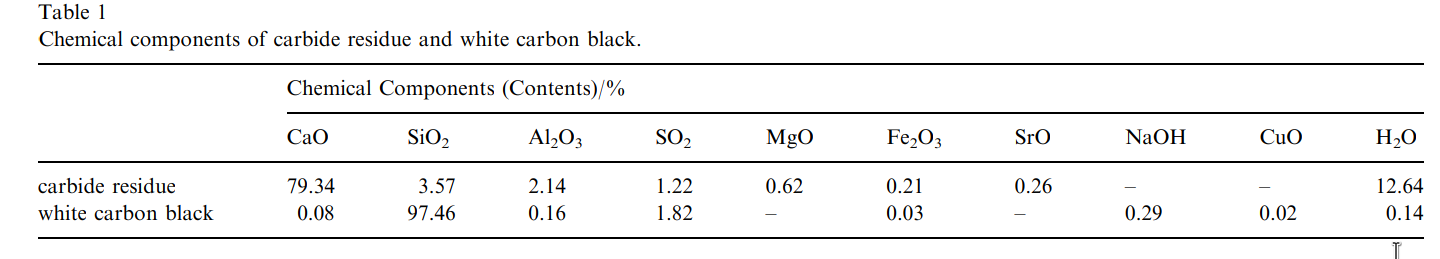
\includegraphics[scale=0.3]{table1.png}

\subsection{表征方法}
\label{sec:org3009fa0}
使用CuKα辐射在XD-2仪器(Persee,China)中收集XRD图案。 在S-4800场发射扫描电子显微镜(日立,日本)上收集FESEM图像。 在ASAP-2010吸附装置(Micromeritics,USA)上通过氮吸附在77.35K下测量BET表面积。

\section{结果和讨论}
\label{sec:org4e54e98}
\subsection{多孔硅酸钙水合物的磷回收性能}
\label{sec:org0755e36}
反应时间对抑制磷浓度的影响如图1所示。在最初的20分钟内观察到磷浓度急剧下降。 随着时间的延长,磷浓度略有下降。 当反应在60分钟达到平衡时,抑制磷浓度的差异是显着的。 当Ca/Si摩尔比为0.6时,抑制磷浓度达到22.19 mg / L. 随着Ca/Si摩尔比的增加,样品的除磷能力显着提高。 当Ca/Si摩尔比为2.2时,抑制磷浓度为2.16mg / L.

图2显示了不同样品投加的磷去除。 当剂量增加时,磷去除效率提高,并且在4000mg / L时获得最高的去除效率。 然后,随着样品剂量的进一步增加,除磷效率几乎保持稳定。 相比较而言,CSH:Ca/Si = 2.2显示出最高的除磷效率。 限制磷浓度仅为2.16 mg / L,沉积物质量为3750 mg。 但是,CSH:Ca/Si = 2.2的磷含量仅为2.6%。 由于磷的去除循环,样品的磷含量可以增加。

\noindent\rule{\textwidth}{0.5pt}
图1.反应时间对抑制磷浓度的影响

\noindent\rule{\textwidth}{0.5pt}
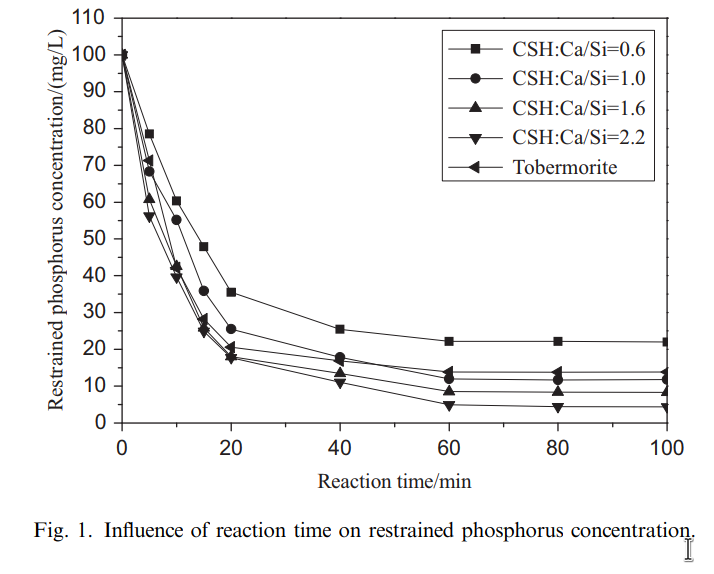
\includegraphics[scale=0.3]{fig.1.png}

\noindent\rule{\textwidth}{0.5pt}
图2.样品用量对抑制磷浓度的影响。

\noindent\rule{\textwidth}{0.5pt}
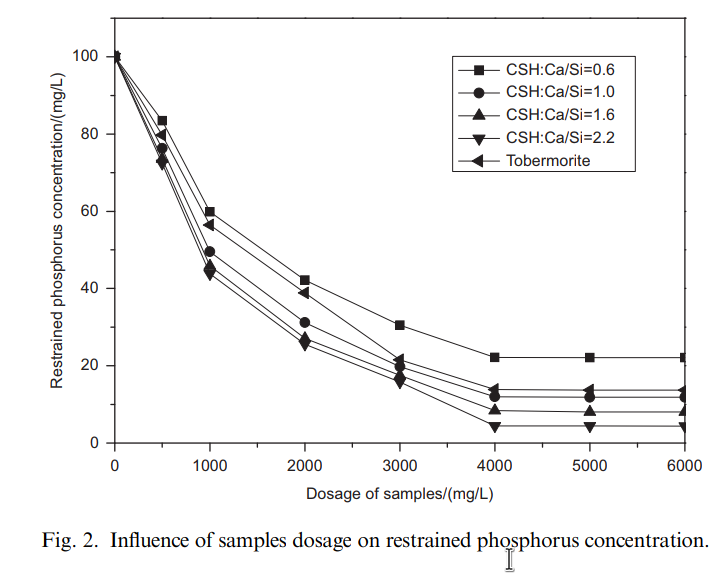
\includegraphics[scale=0.3]{fig.2.png}

\noindent\rule{\textwidth}{0.5pt}
图3.除磷循环抑制磷浓度的变化。

\noindent\rule{\textwidth}{0.5pt}
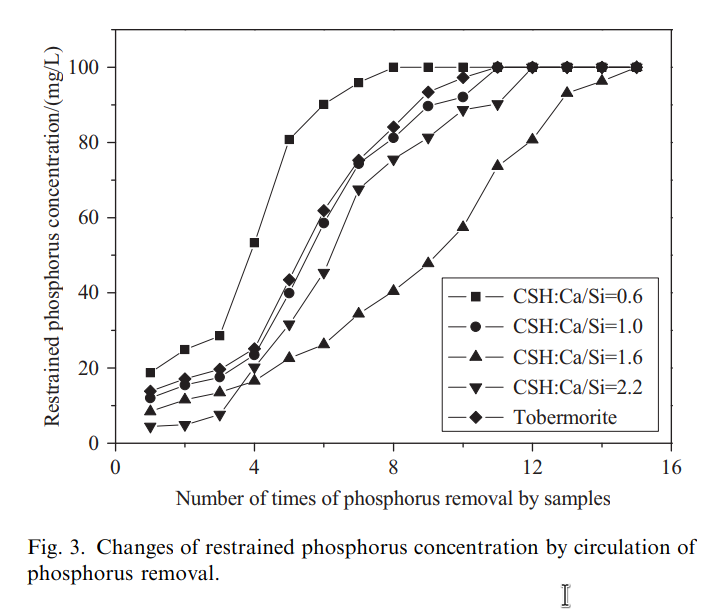
\includegraphics[scale=0.5]{fig.3.png}

从除去的合成溶液中分离样品,然后加入初始磷浓度为100mg / L的合成溶液中。抑制磷浓度的变化如图3所示.CSH的除磷性能:Ca/Si = 2.2在前3次保持良好,在第12次后停止。 CSH:Ca/Si = 2.2的磷含量为14.10%,而CSH:Ca/Si = 1.6的磷含量达到18.64%。 CSH:与CSH相比,Ca/Si = 1.6具有更高的磷回收性能:Ca/Si = 2.2。样品的磷去除性能与pH值有关。随着磷去除时间的延长,pH值降低(图4)。如图所示,CSH:Ca/Si = 2.2在前3次引起一系列高pH值(pH = 9.8 10.2),并在第4次(pH = 8.5)急剧下降。 CSH:Ca/Si = 1.6可以长时间保持高pH值(pH = 8.5-9.5)(去除磷的10倍)。这种条件有利于除磷循环。

\subsection{多孔硅酸钙水合物的孔结构}
\label{sec:org6f134f6}
样品上的氮吸附 - 解吸等温线如图5所示。结果表明吸附滞后环现象。 这意味着样品上存
在中孔或窄间隙孔\cite{Poreestructure_and_surface_fractal_characteristics_of_calcium_silicate_hydrates_contained_organic_macromolecule}。 在mespore中的吸附主要发生在中压区域(0:4op = p0o0:9)。
随着Ca/Si摩尔比的增加,吸附磁滞回线现象变得明显,吸附曲线增大。 CSH的比表面积:
Ca/Si = 0.6,CSH:Ca/Si = 1.0,CSH:Ca/Si = 1.6,CSH:Ca/Si = 2.2和雪硅
钙石分别为11.91,59.67,113.36,121.03和49.85m2 / g ,分别。这些样品的孔体积相应
地为0.07,0.30,0.52,0.65和0.15cm 3 / g。 Ca/Si摩尔比的增加导致孔径更小,比表面积和孔体积更大。

通过FESEM观察和EDS分析检查了雪硅钙石的表面结构,CSH:Ca/Si = 1.6和CSH:Ca/Si = 2.2(图6)。 与雪硅钙石相比,CSH:Ca/Si = 1.6具有正面的纤维网络结构,具有大量的中孔。 CSH:Ca/Si = 2.2除了纤维网络结构外还有大块的片状晶体。 EDS分析证实,雪硅钙石的粗糙表面,CSH:Ca/Si = 1.6和CSH:Ca/Si = 2.2主要由Ca和Si组成。 Ca/Si摩尔比分别为0.8,1.5和2.0。 由于在过滤浆料时部分Ca \^{}\{2+\}的损失,合成后材料的Ca/Si摩尔比降低。 因此,CSH的单一除磷效率随着比表面积的增加而增加。

\noindent\rule{\textwidth}{0.5pt}

图4.除磷循环对pH值的影响。

\noindent\rule{\textwidth}{0.5pt}
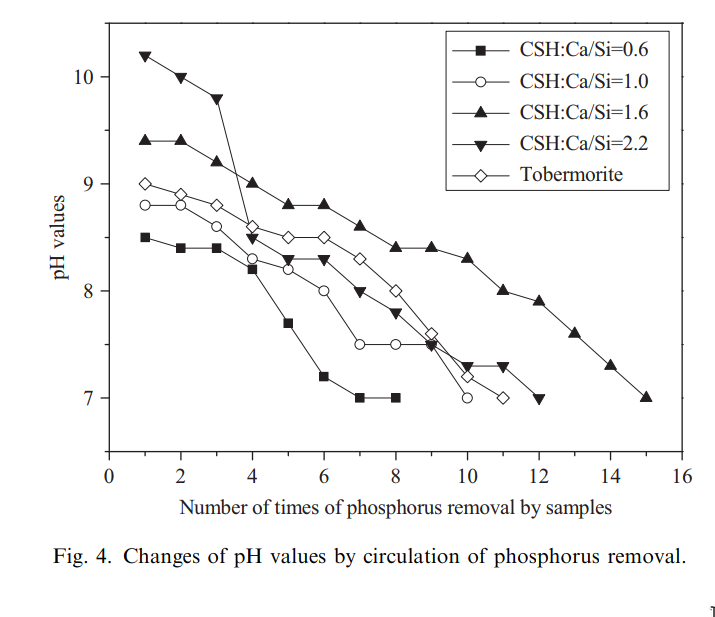
\includegraphics[scale=0.5]{fig.4.png}

\noindent\rule{\textwidth}{0.5pt}
图5.样品上的氮吸附 - 解吸等温线

\noindent\rule{\textwidth}{0.5pt}
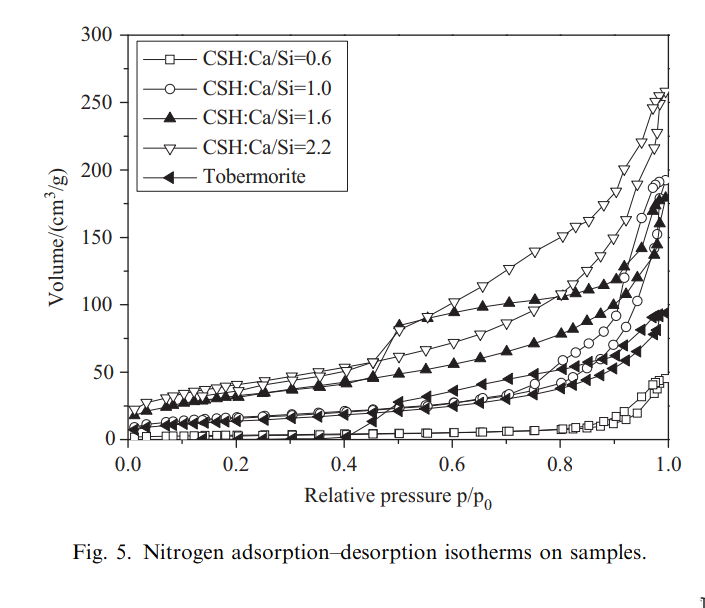
\includegraphics[scale=0.5]{fig.5.png}

\noindent\rule{\textwidth}{0.5pt}
图5.FESEM观察和EDS分析。 (a)雪硅钙石表面; (b)雪硅钙石的化学分析; (c)CSH表面:Ca / Si = 1.6; (d)CSH的化学分析:Ca / Si = 1.6; (e)CSH表面:Ca / Si = 2.2; (f):CSH的化学分析:Ca / Si = 2.2。

\noindent\rule{\textwidth}{0.5pt}
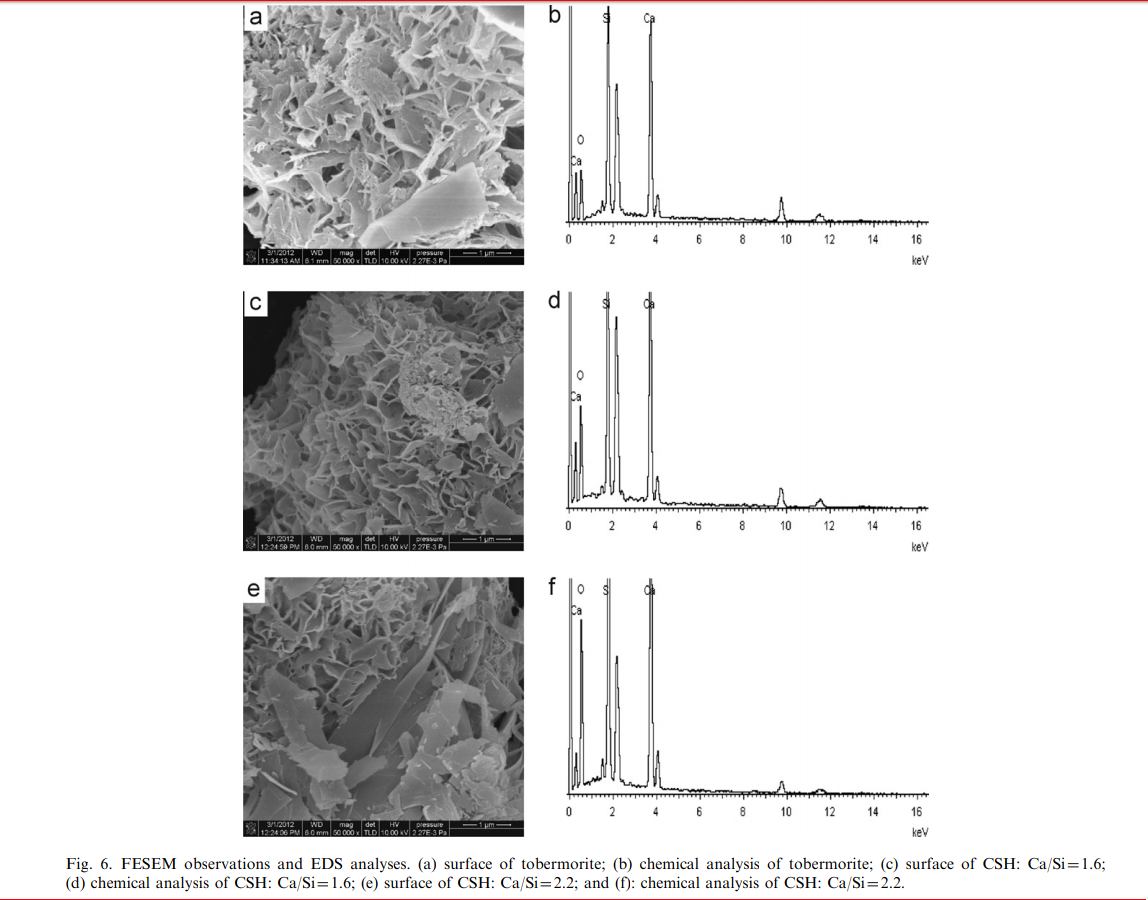
\includegraphics[scale=0.5]{fig.6.png}

\noindent\rule{\textwidth}{0.5pt}
\subsection{Ca\textsuperscript{2+}释放动力学}
\label{sec:orgfec6faf}
实验表明,Ca\textsuperscript{2+}浓度随着Ca/Si摩尔比的增加而增加(图7)。 从雪硅钙石释放的
Ca\textsuperscript{2+}浓度,CSH:Ca/Si = 1.6和CSH:Ca/Si = 2.2分别为2.10,3.56,4.91mg / g。
根据Avrami动力学模型方程(方程(2)绘制Ca\textsuperscript{2 +}释放的实验能力。\cite{demirkıran07_dissol_kinet_ulexit_perch_acid_solut}

\[-\ln(1-x) = kt^{n} \ \ \ (2)\]

其中k是动力学常数,n是固体的特征常数,t是反应时间(min)和x(x¼Ct/ C\textsubscript{max},Ct是时间t的浓度(mg / L),C\textsubscript{max}是最大浓度(mg) / L))是分数转换。 特征常数n为0.9019。 通过将Avrami动力学模型拟合到从图6(表2)获得的实验数据来确定动力学常数。 高相关系数(R2> 0.99)表明该模型可以很好地描述Ca\textsuperscript{2+}释放规律。


如表2所示,随着Ca/Si摩尔比的增加,k变大。 结合材料的比表面积(S),可以建立k和S之间的关系(方程(3))。

\[k = 0.022S^{0.292} \ \ R = 0.9135 \ \ \ (3)\]

根据Eq。 (3)样品的比表面积和Ca\textsuperscript{2+}释放速率相互吻合良好。 通过用Eq。代替,得到比表面积与Ca\textsuperscript{2+}溶解浓度之间的关系。 (3)进入Eq。(2)。

\[-\ln(1-x) = 0.022S^{0.292}t^{0.9019} \ \ \ (4)\]

根据Eq。 (4),Ca\textsuperscript{2+}释放浓度与比表面积有关。 该结果证明了Ca/Si摩尔比对磷回收能力的影响。 Ca/Si摩尔比影响孔结构和Ca\textsuperscript{2+}释放能力。 由于比表面积较大,Ca\textsuperscript{2+}释放得更快。 多孔结构提供了维持高浓度Ca\{2+\}释放的局部条件。 比较CSH:Ca/Si = 1.6与CSH:Ca/Si = 2.2,前者具有较高的磷回收性能。 因此,Ca\textsuperscript{2+}释放规律是磷回收性能的关键。 CSH:Ca/Si = 1.6可以释放适当浓度的Ca\textsuperscript{2+}和OH\textsuperscript{-}以维持pH值在8.5-9.5之间。 磷酸盐以这些pH值范围内的HPO\textsuperscript{2-}\textsubscript{4}形式存在。\cite{liu12_remov_high_concen_phosp_by_calcit} Ca\textsuperscript{2+},OH\textsuperscript{-}和HPO\textsuperscript{2-}\textsubscript{4}形成高浓度的局部条件。 这种条件有利于羟基磷灰石的形成,pH = 8.5-9.5。


可以通过XRD进一步研究该机理。比较样品的XRD图谱(图8)。当Ca/Si摩尔比为0.6:1和1:1时,生产硬硅钙石(PDF卡23 0125,化学式Ca\textsubscript{6}Si\textsubscript{6}O\textsubscript{17}(OH)\textsubscript{2})。对于CSH:Ca/Si = 0.6,SiO 2的主峰出现在20.3051和21.5621。 CSH中的主峰:Ca/Si = 1.6和CSH:Ca/Si = 2.2归属于jennite(PDF卡18-1206;式Ca\textsubscript{9}Si\textsubscript{6}O\textsubscript{18}(OH)\textsubscript{6}·8H2O;理论Ca/Si摩尔比为1.5)。 CSH:Ca/Si = 2.2的XRD图谱显示存在Ca(OH)\textsubscript{2}。形成的Ca(OH)\textsubscript{2}的覆盖率与基于FESEM观察的结果完全一致[27]。

\noindent\rule{\textwidth}{0.5pt}
图7.样品中释放的Ca2 +浓度。

\noindent\rule{\textwidth}{0.5pt}
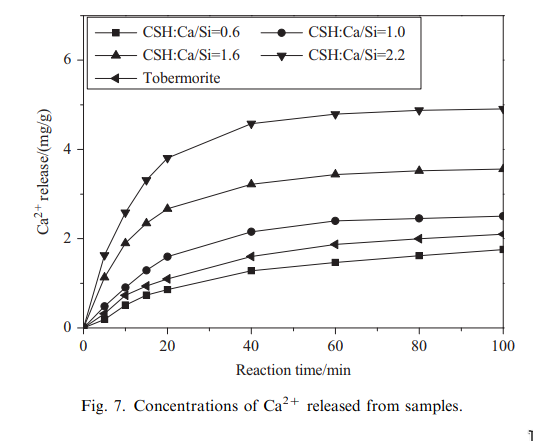
\includegraphics[scale=0.5]{fig.7.png}

\noindent\rule{\textwidth}{0.5pt}
图8.样品的X射线衍射(XRD)图案

\noindent\rule{\textwidth}{0.5pt}
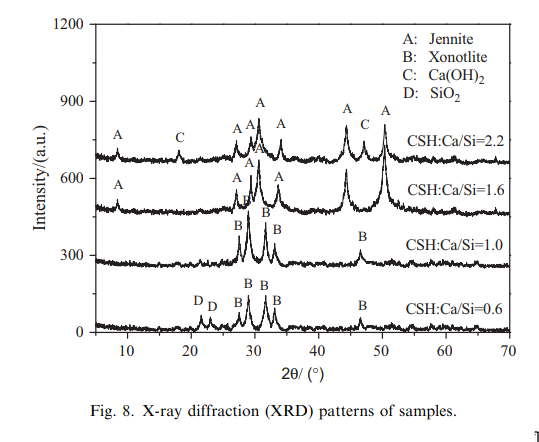
\includegraphics[scale=0.5]{fig.8.png}

\noindent\rule{\textwidth}{0.5pt}

实验表明,与硬硅钙石和雪硅钙石相比,jennite具有更强的Ca\textsuperscript{2+}释放能力。低Ca/Si
摩尔比导致白炭黑过剩。因此,在材料表面上形成富含Si的层并阻止Ca\textsuperscript{2+}释放。随后,
材料的磷回收能力下降。 Ca(OH)\textsubscript{2}的形成是由于具有高Ca/Si摩尔比的碳化物残余物的
过剩。由于Ca(OH)\textsubscript{2}的存在,CSH的单磷去除效率:Ca/Si = 2.2优于其他样品。然而,
大量的Ca\textsuperscript{2+}被释放并与浸入合成溶液中的材料一样快地与磷酸根离子反应。羟基磷灰石层在短时间内形成并导致孔结构的阻塞。因此Ca\textsuperscript{2+}释放能力下降。

\section{总结}
\label{sec:org1424aba}
采用动态水热法,采用碳化物残渣和白炭黑合成了多孔硅酸钙水合物。 Ca/Si摩尔比对多孔硅酸钙水合物的磷回收性能产生显着影响。 多孔硅酸钙水合物的Ca/Si摩尔比为1.6更适合回收磷。 多孔硅酸钙水合物可以回收磷,磷含量为18.64%。


Ca\textsuperscript{2+}和OH\textsuperscript{-}释放规律是磷回收效率的关键。 Ca/Si摩尔比的变化导致不同的孔结构。 比表面积的增加和Ca\textsuperscript{2+}释放浓度的增加彼此非常一致。


XRD的进一步分析表明,两种情况影响了Ca\textsuperscript{2+}释放规律。 一方面,低Ca/Si摩尔比导致形成富Si层。 另一方面,Ca(OH)\textsubscript{2}由于高Ca/Si摩尔比而形成。


\bibliography{man}
\bibliographystyle{alpha}
\end{document}
